\section{DFDs}
A data flow diagram (DFD) is a graphical representation of the "flow" of data through an information system, modeling its process aspects. A DFD is often used as a preliminary step to create an overview of the system, which can later be elaborated. DFDs of DoS is as following-:
\begin{enumerate}
\item Data flow LEVEL 0 figure \ref{fig:DFDs}
\item Data flow LEVEL 1 figure \ref{fig:DFDs1}
\end{enumerate}

\begin{figure}[H]
\centering 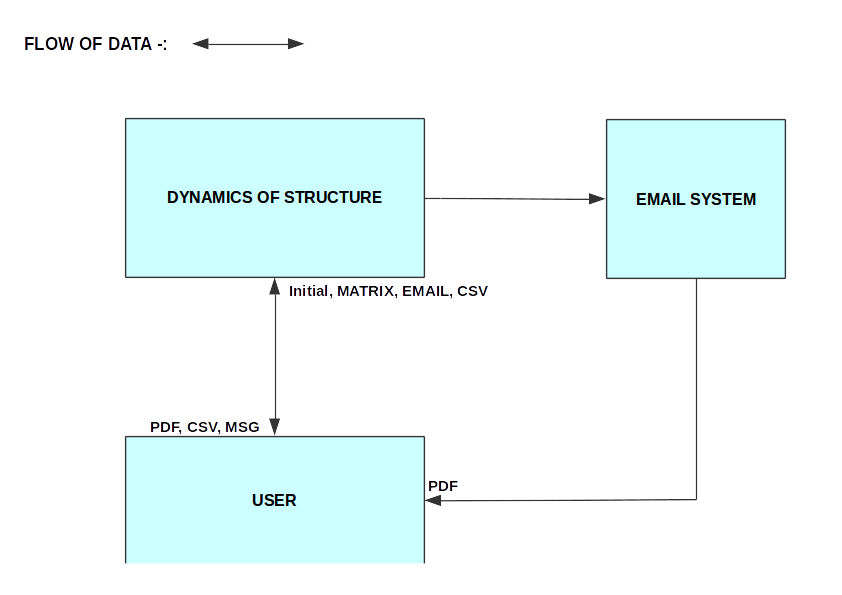
\includegraphics[scale=0.4]{images/DFDS.png}
\caption{Data flow LEVEL 0}
\label{fig:DFDs}
\end{figure}
Here, In figure \ref{fig:DFDs} and figure \ref{fig:DFDs1}
\begin{enumerate}
\item MSG means Message
\item initial represent all initial input value
\item matrix represent all Mass, Height, Stiffness matrix
\end{enumerate}
\begin{figure}[H]
\centering 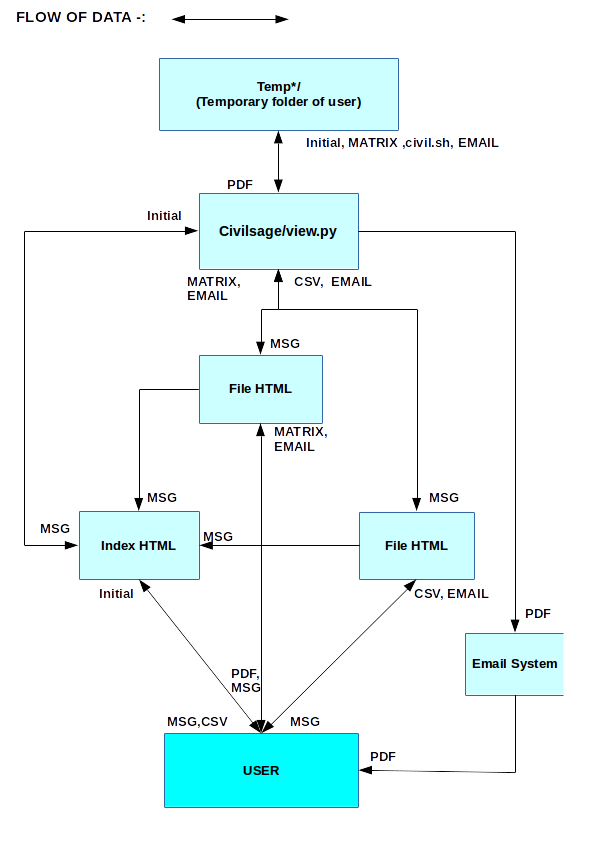
\includegraphics[scale=0.55]{images/DFDS1.png}
\caption{Data Flow LEVEL 1}
\label{fig:DFDs1}
\end{figure}
\section{UI Flow Diagram}
UI Flow diagram tells how user will perceive different interface on click of different buttons or trigger. The rectangular blocks represent entities and Arrow represents change of view from one to another on the bases of button clicked mentioned near arrow.UI flow Diagram of DoS is given below figure \ref{fig:UI1} -: 
\begin{figure}[H]
\centering 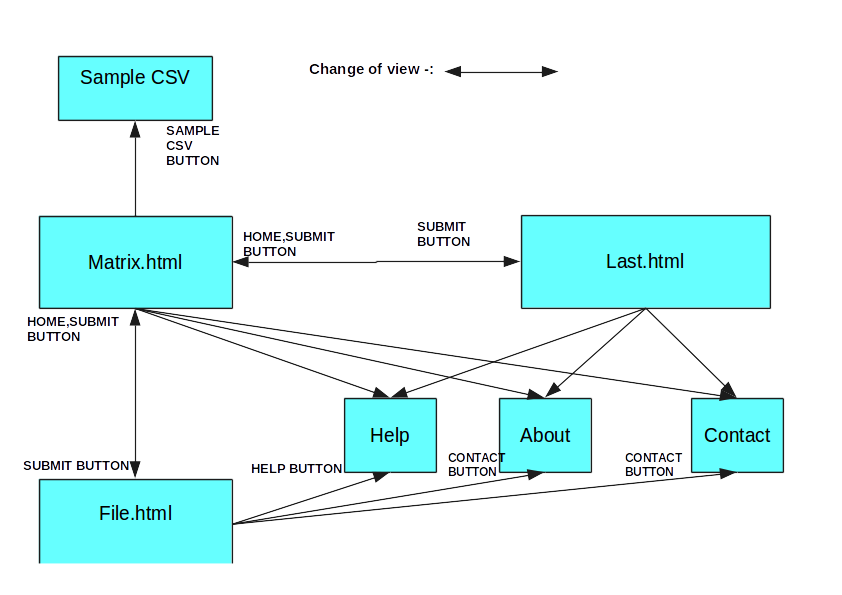
\includegraphics[scale=0.55]{images/UI.png}
\caption{UI Flow diagram}
\label{fig:UI1}
\end{figure}
\section{Flowchart}
A flowchart is a type of diagram that represents an algorithm, work flow or process, showing the steps as boxes of various kinds, and their order by connecting them with arrows
and following are flowchart of DoS showing flow of control and Data in the software-:

Figure \ref{fig:FD1} give flow of whole system with flow of mentioned modules explained at -:
\begin{enumerate}
\item view.matrix() \ref{fig:FD1}
\item initialfile.emailpdf() \ref{fig:FD}
\item view.last() at figure \ref{fig:FD2}
\item view.file() at figure \ref{fig:FD3}
\item view.pdfemail() at figure \ref{fig:FD4}
\end{enumerate}
Here, In figure \ref{fig:FD}
\begin{enumerate}
\item Initial input represent all initial input value given in home page
\item MLS represent all Mass, Height(level), Stiffness matrix
\end{enumerate}

\begin{figure}[H]
\centering 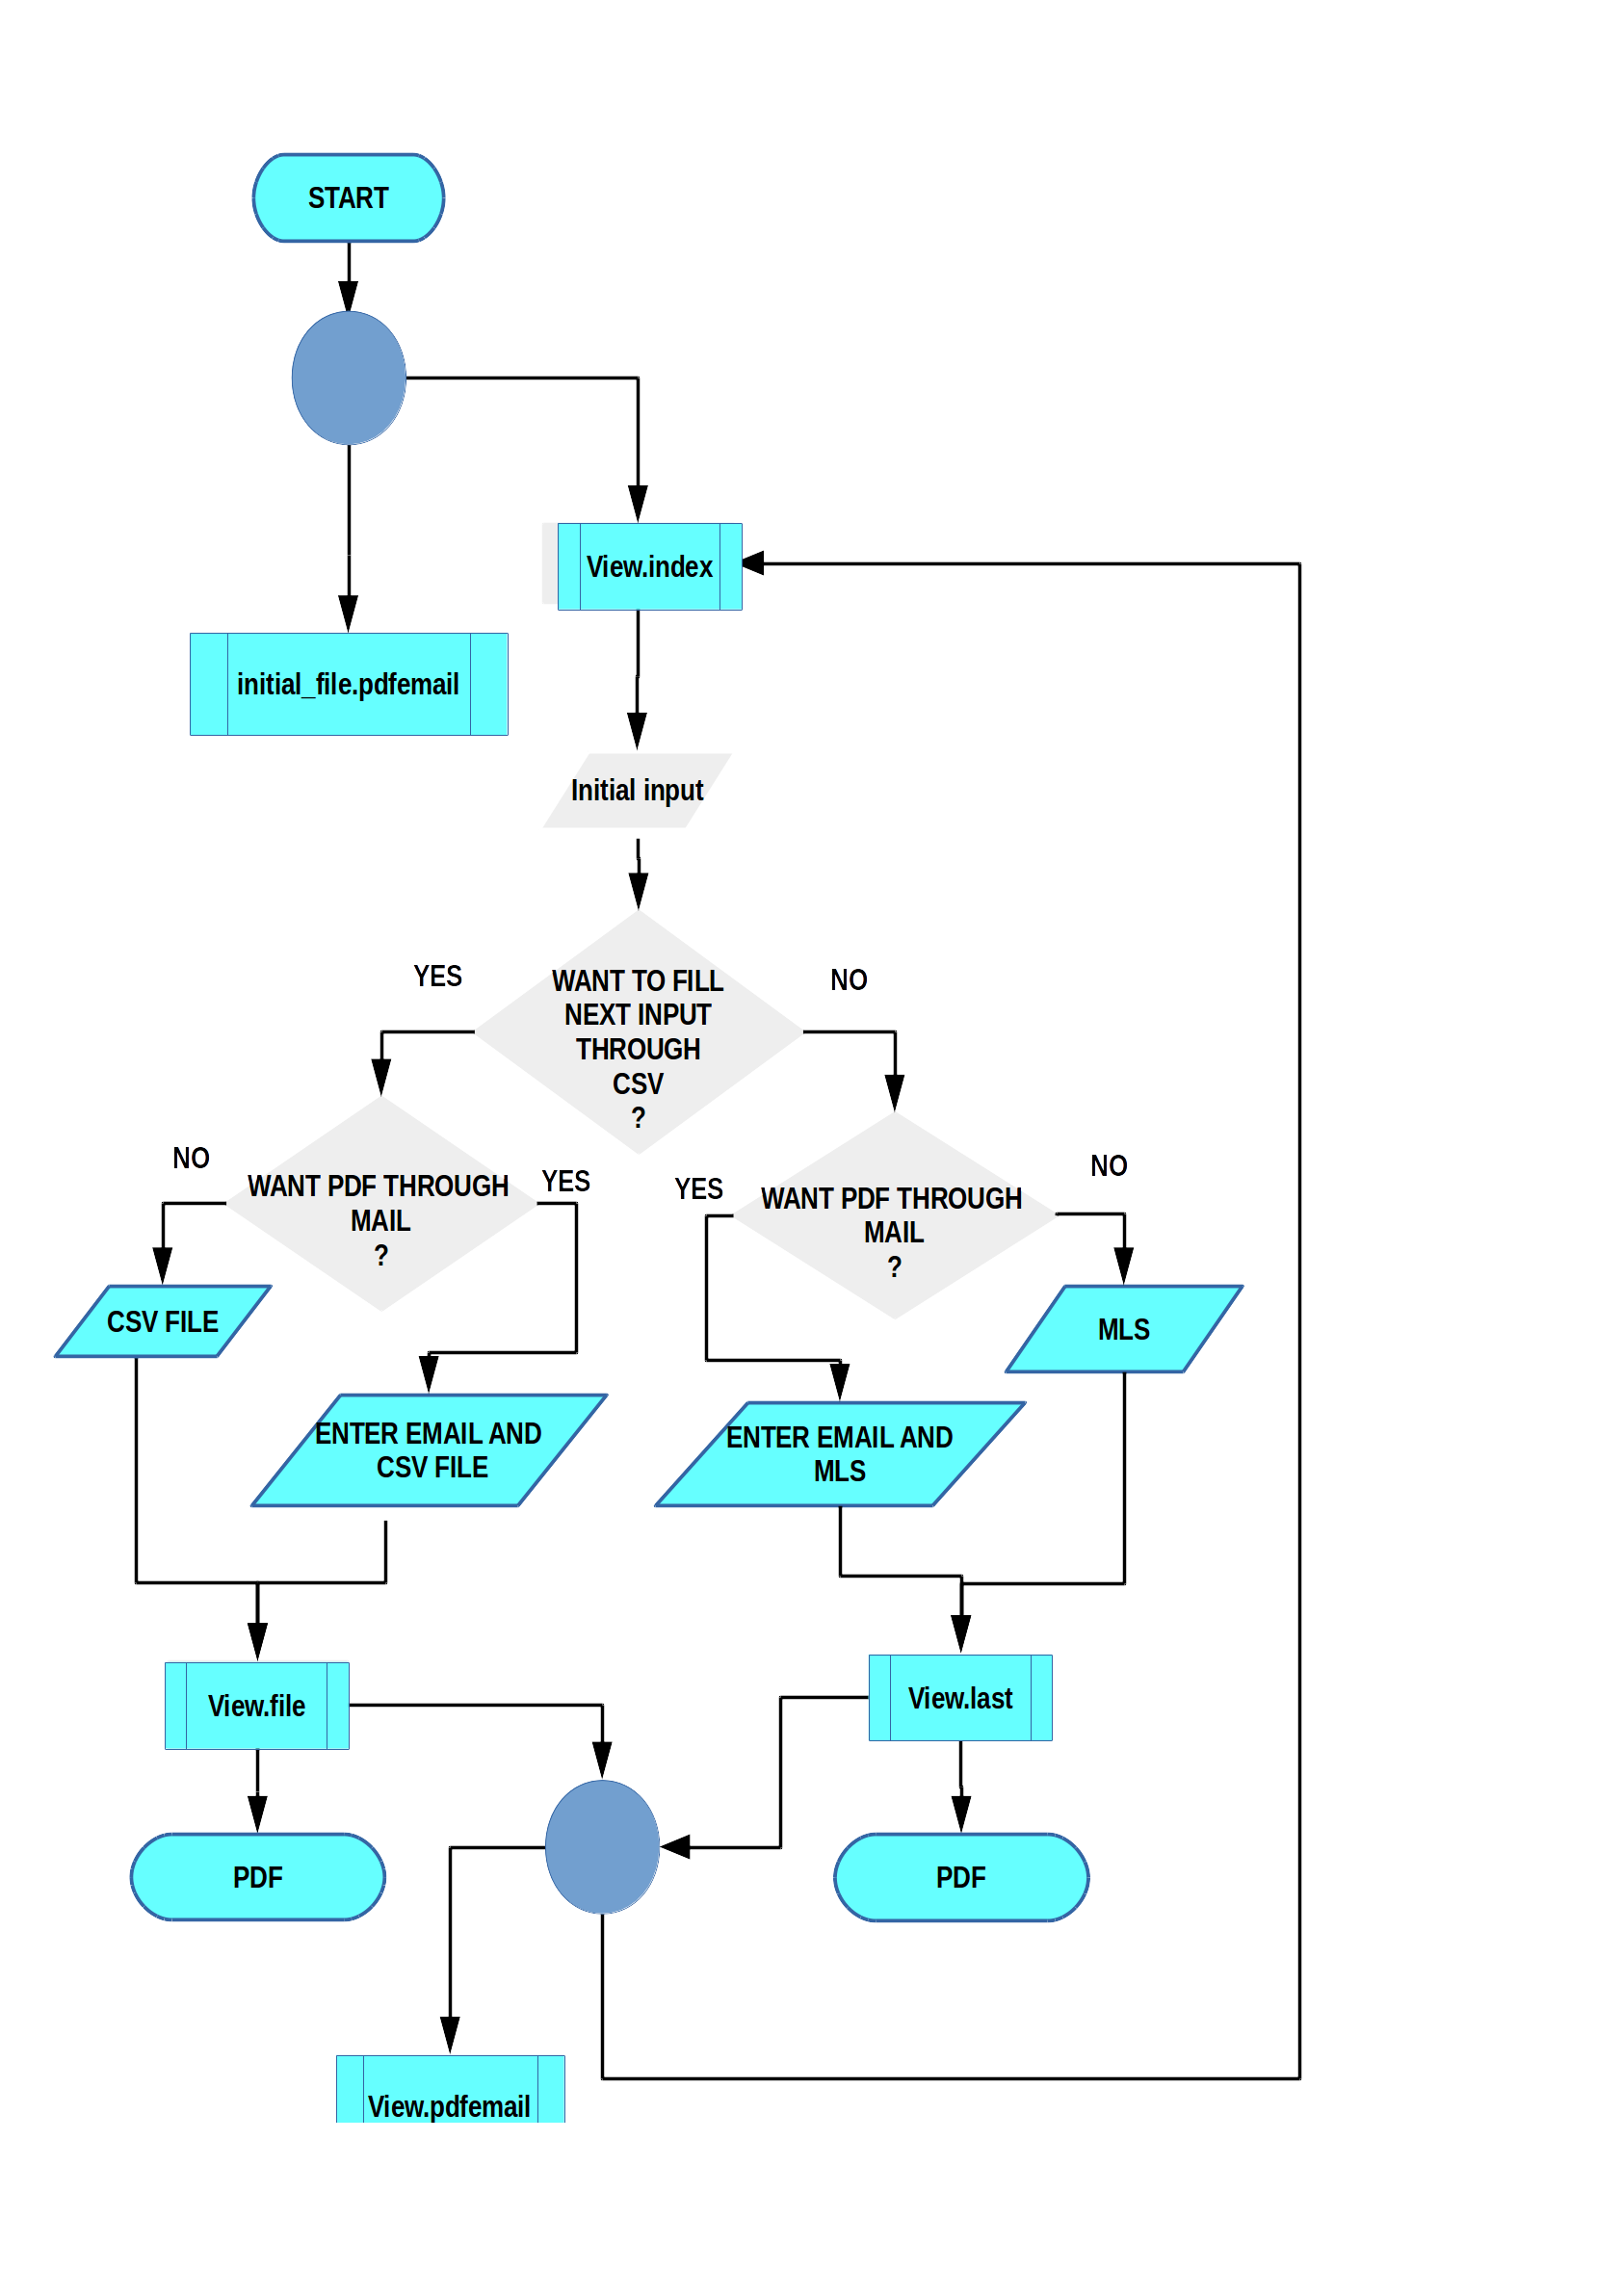
\includegraphics[scale=0.27]{images/flowchart.png}
\caption{Flowchart of Whole System}
\label{fig:FD1}
\end{figure}

\begin{figure}[H]
\centering 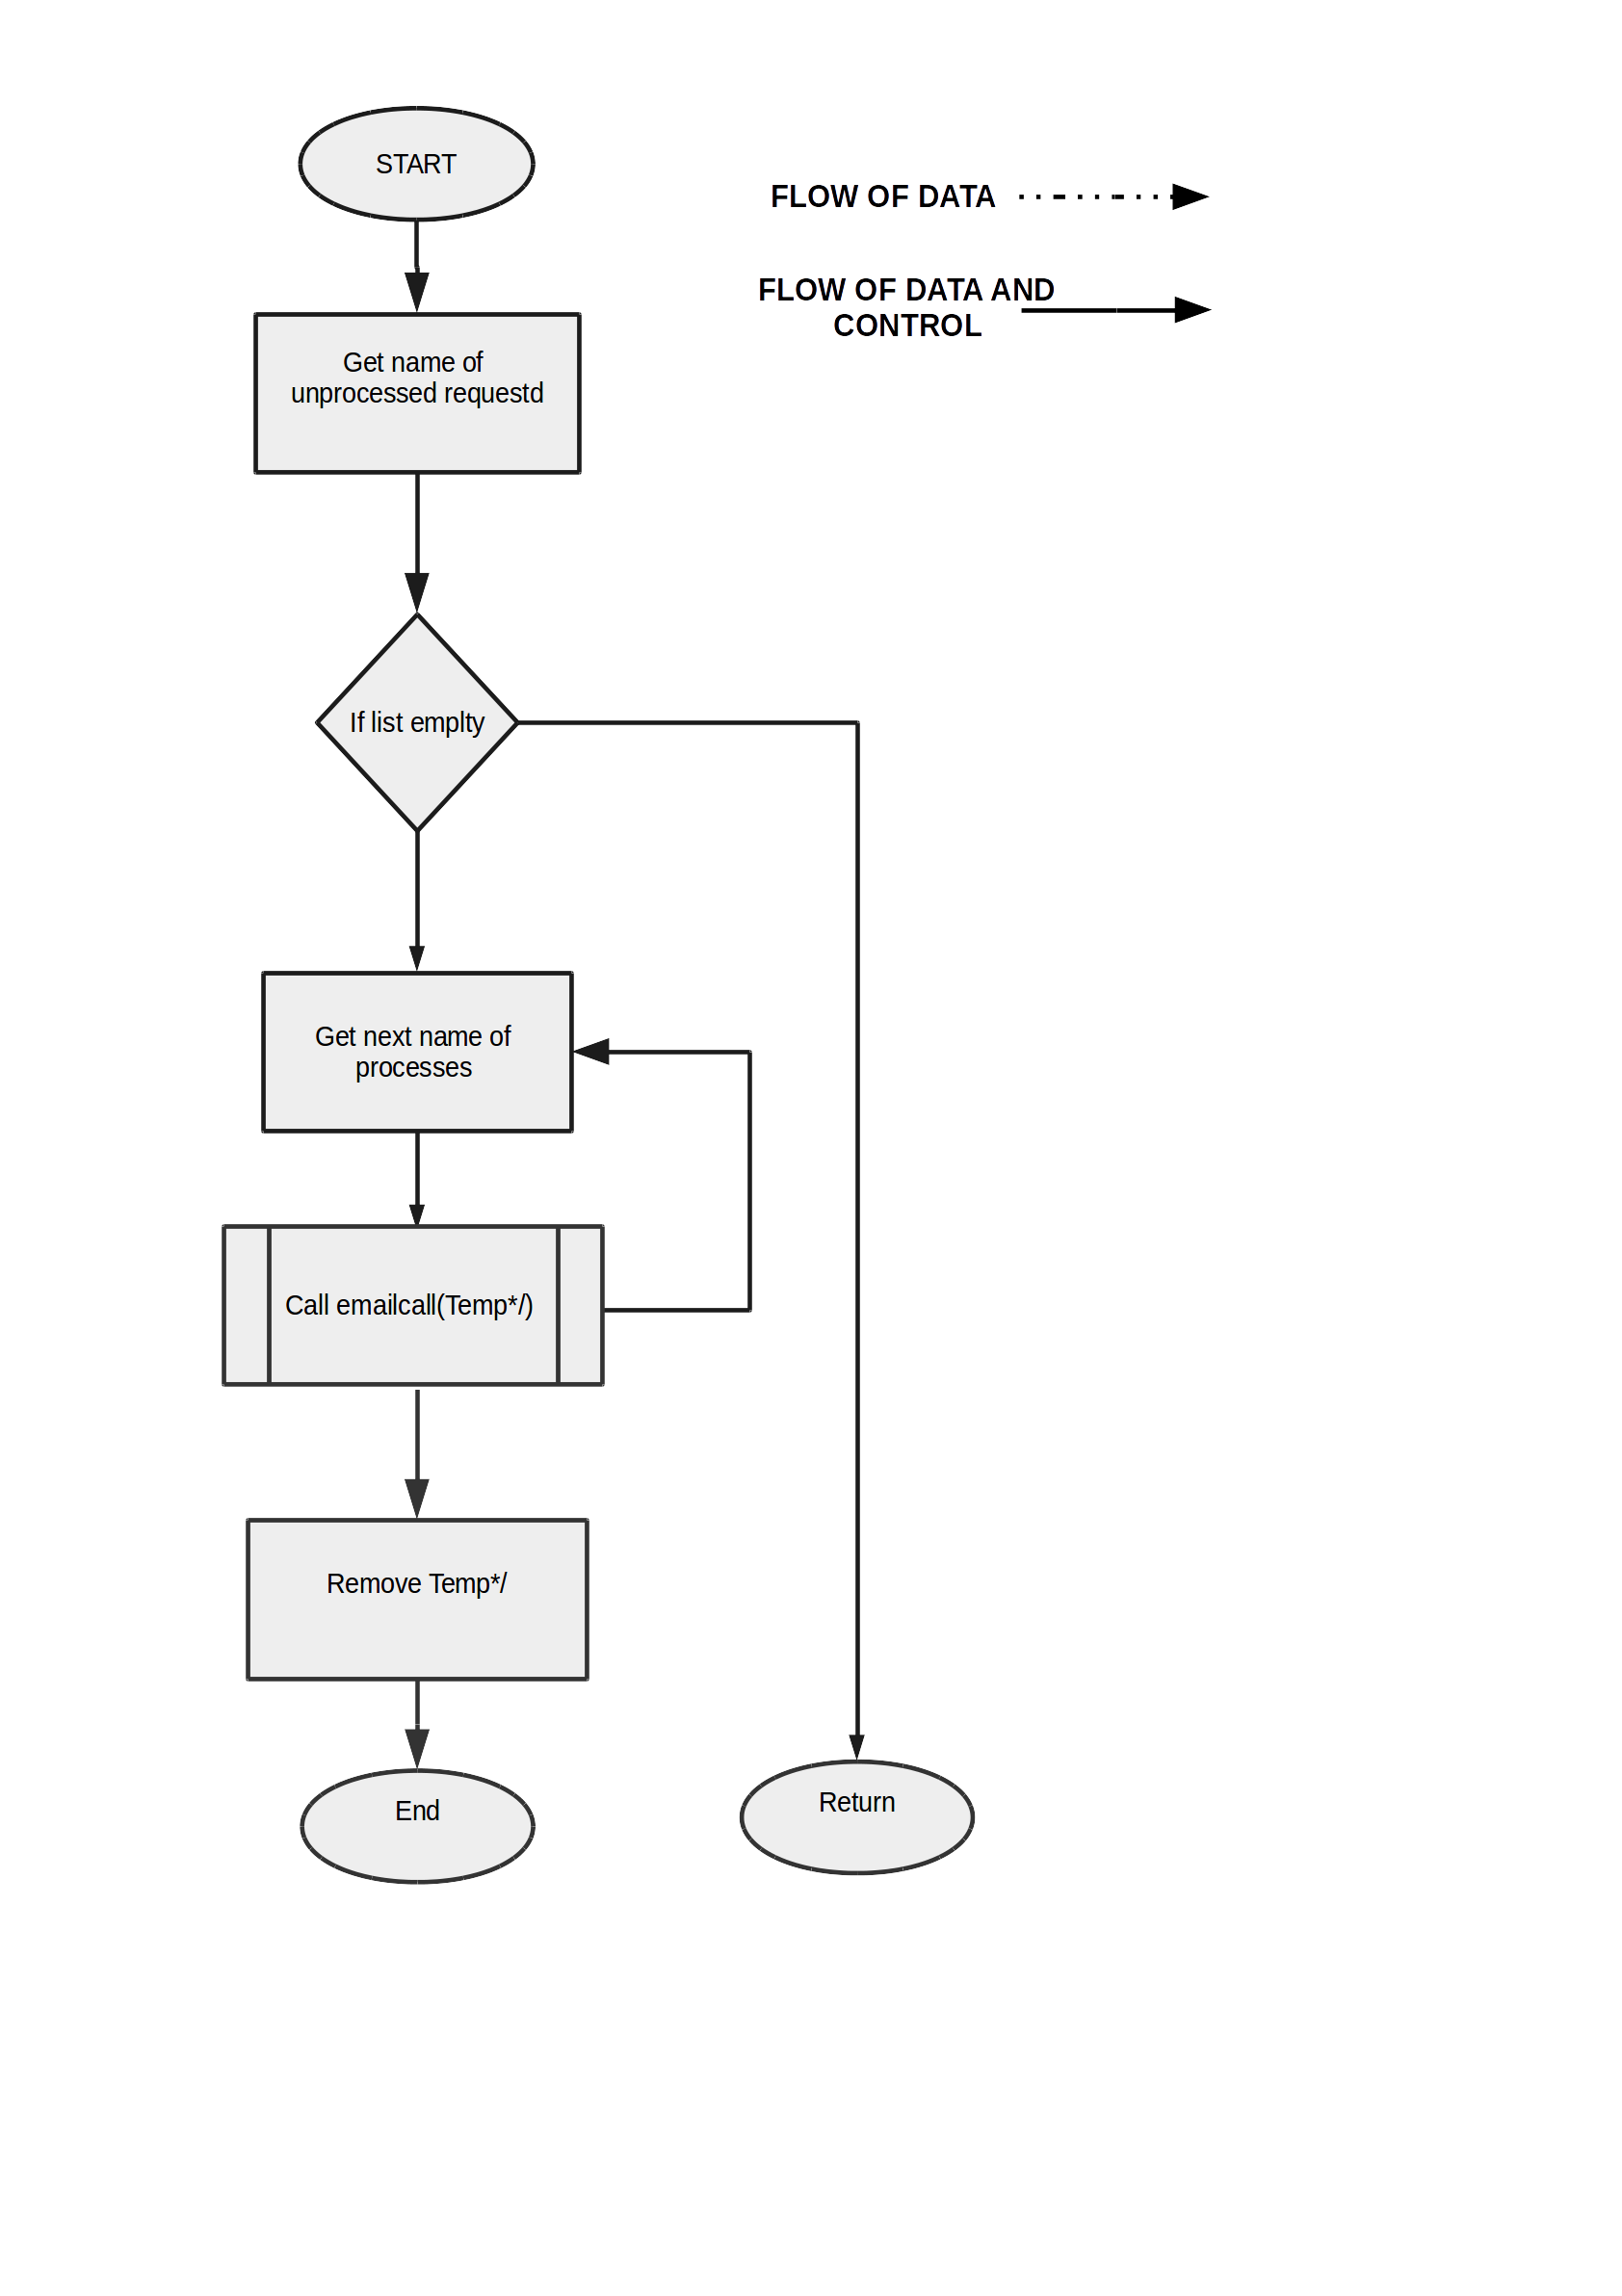
\includegraphics[scale=0.27]{images/flowchartm.png}
\caption{Flowchart of initialfile.pdfemail()}
\label{fig:FD}
\end{figure}

\begin{figure}[H]
\centering 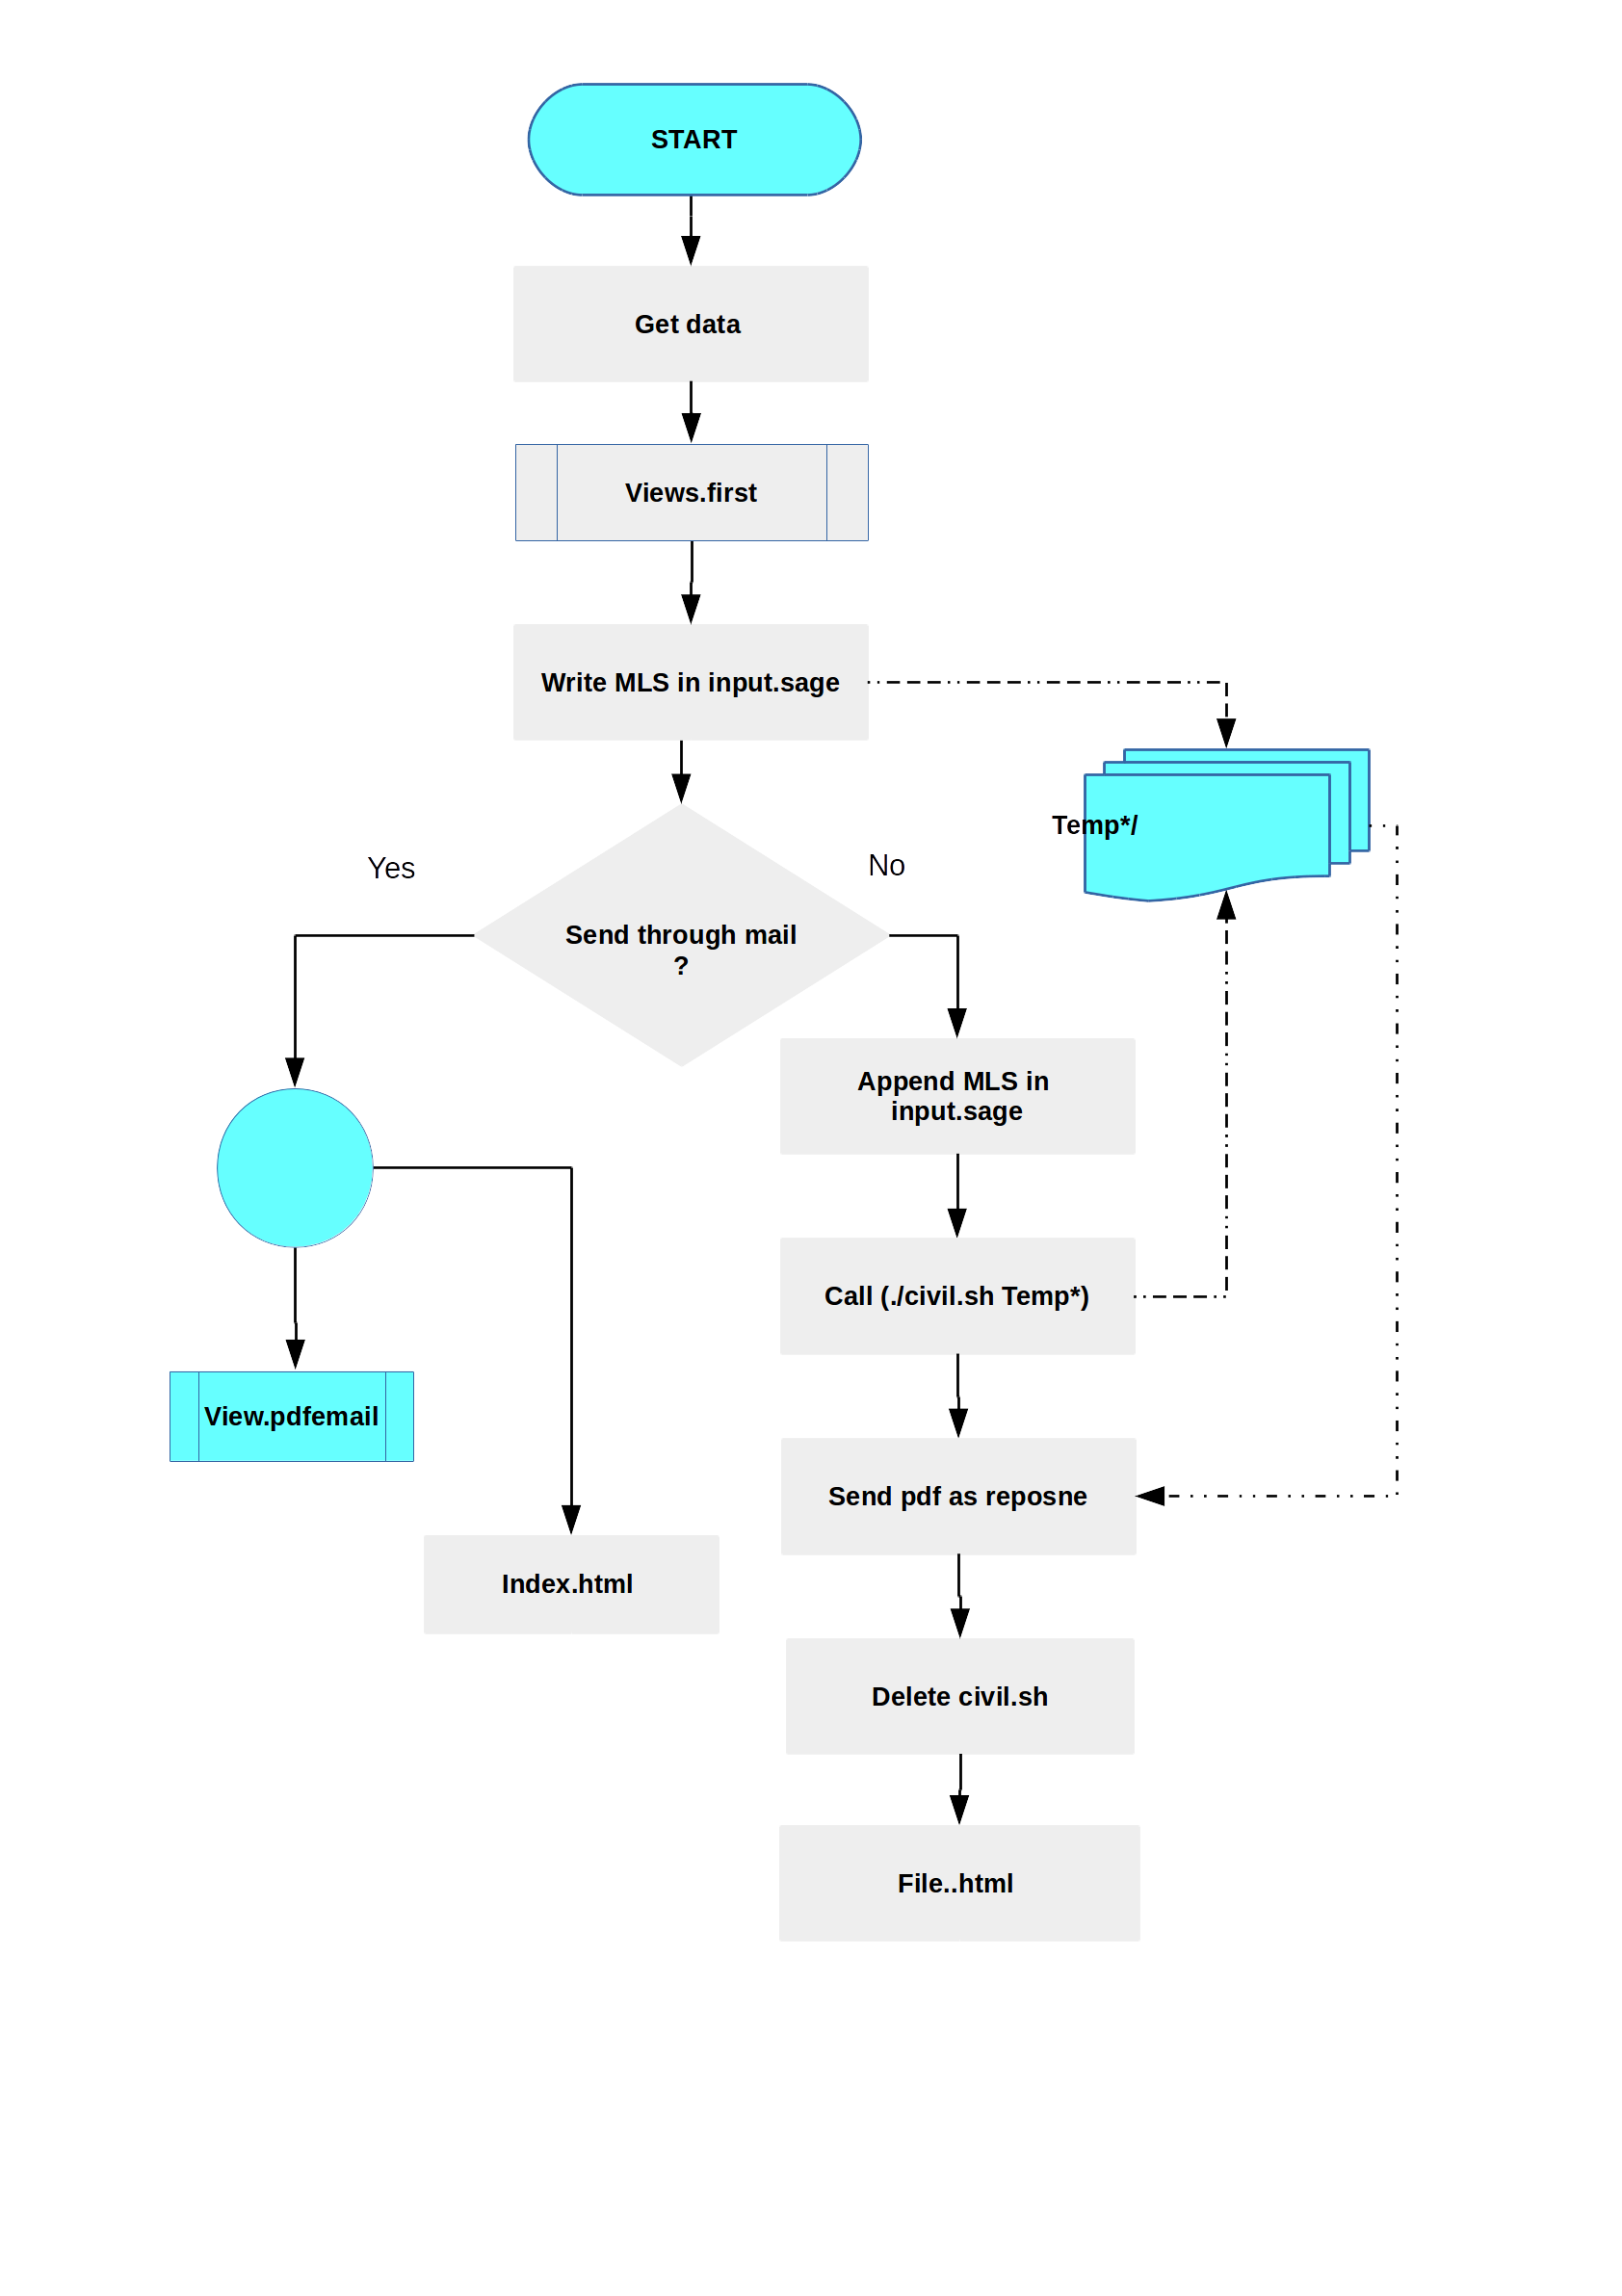
\includegraphics[scale=0.27]{images/flowchartmatrix.png}
\caption{Flowchart of veiw.last()}
\label{fig:FD2}
\end{figure}
\begin{figure}[H]
\centering 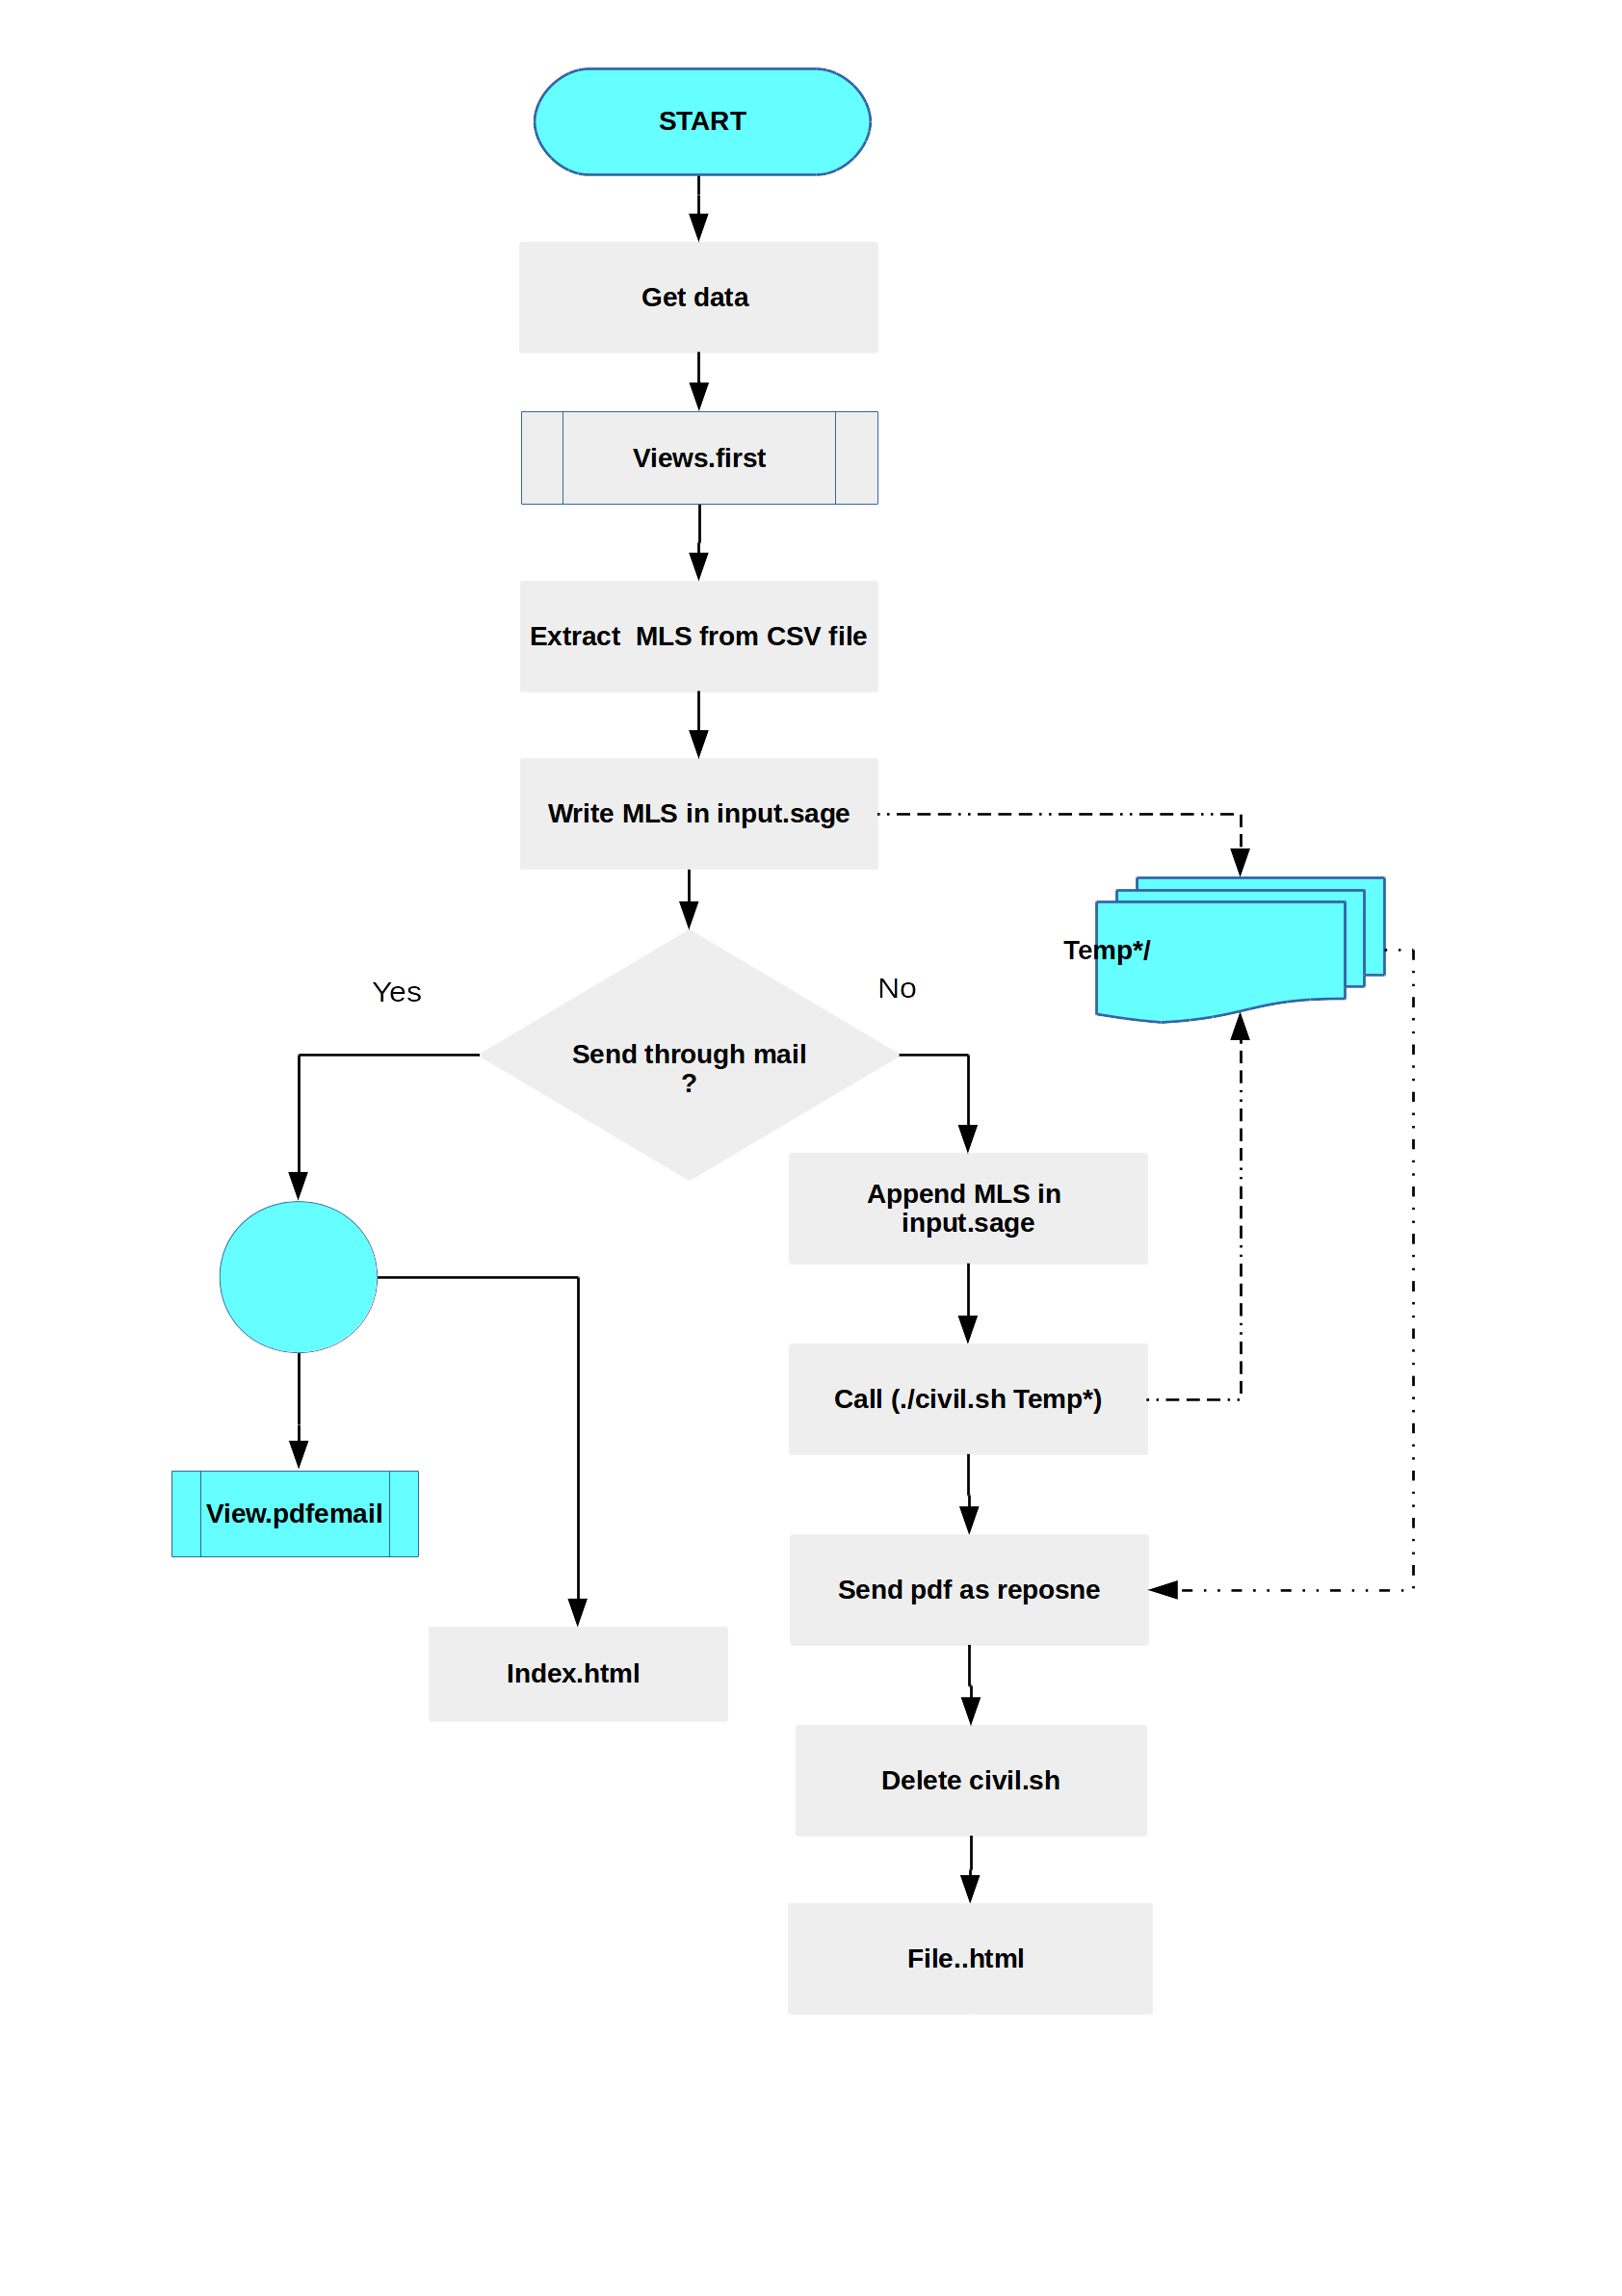
\includegraphics[scale=0.27]{images/flowchartfile.png}
\caption{Flowchart of veiw.file()}
\label{fig:FD3}
\end{figure}
\begin{figure}[H]
\centering 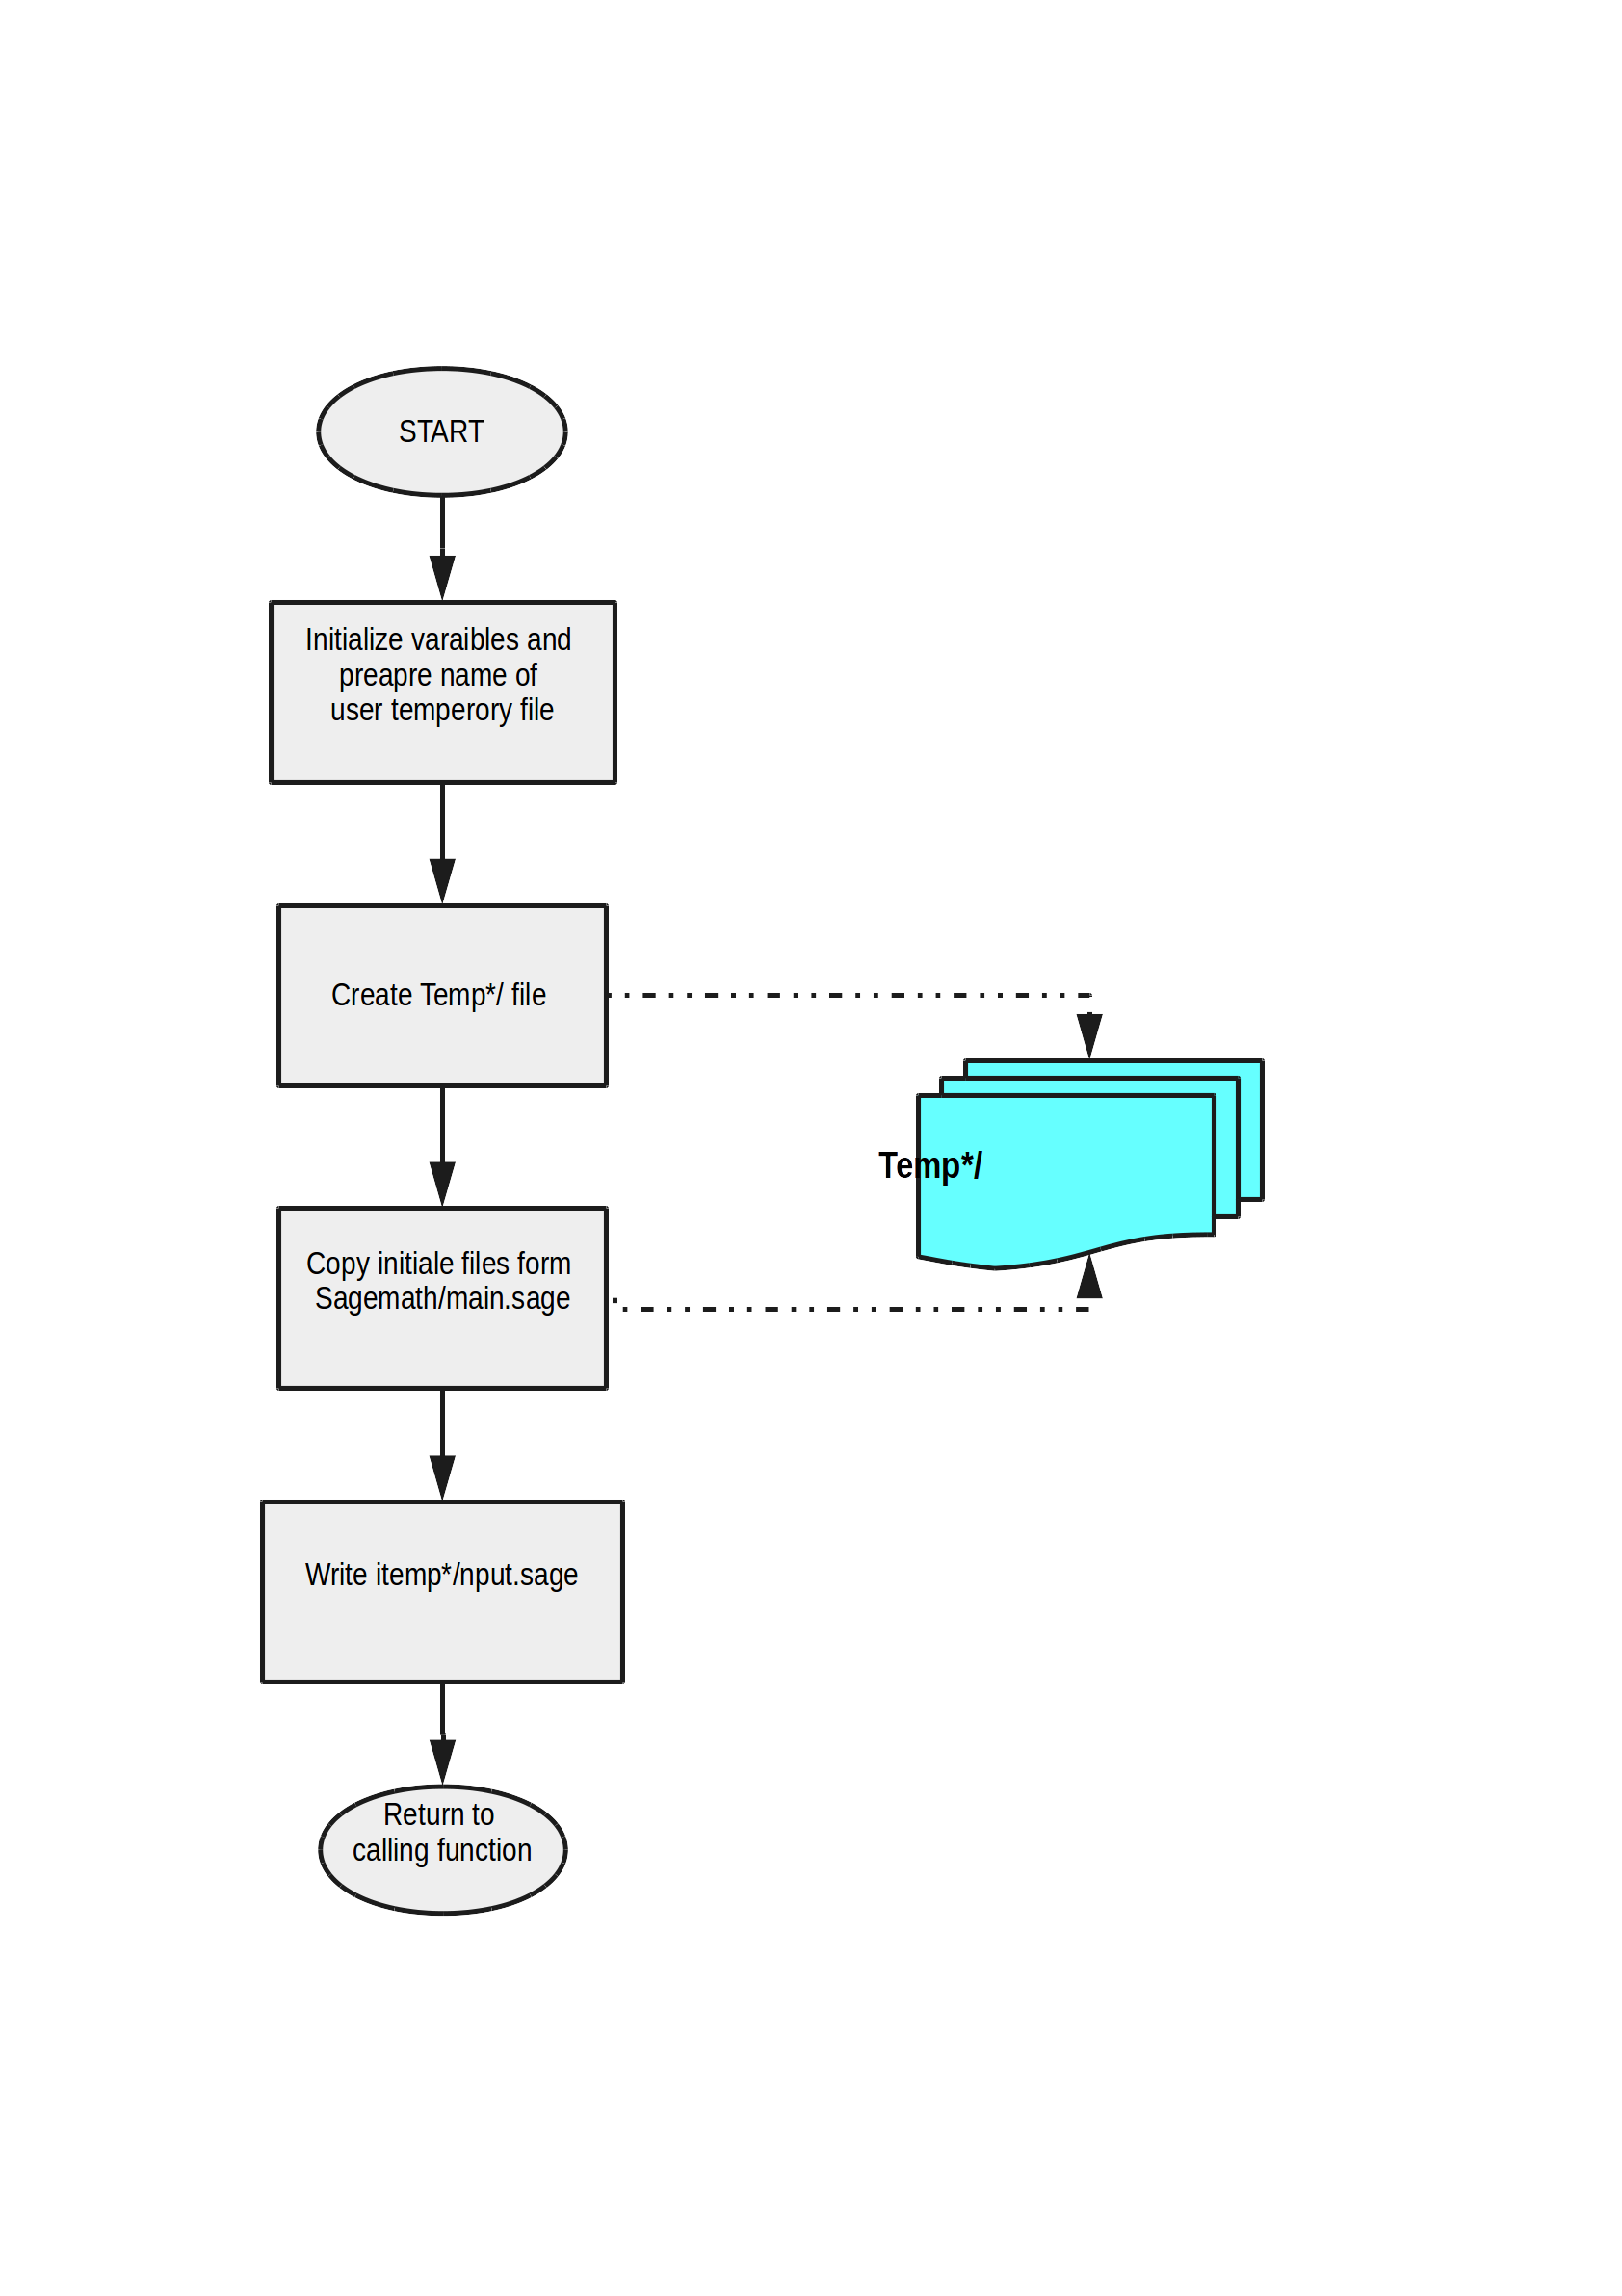
\includegraphics[scale=0.27]{images/flowchartpdf.png}
\caption{Flowchart of veiw.pdfemail()}
\label{fig:FD4}
\end{figure}


